
\par $S_{cheio_{fome}} = [2,2]$

\vskip 0.1in
\par $S_{alternativa^+} = [2,2]$
\par $Ganho(S_{cheio_{fome}}, S_{alternativa}) = 0$

\vskip 0.1in
\par $S_{bar^+} = [1,1]$  \qquad $S_{bar^-} = [1,1]$
\par $Ganho(S_{cheio_{fome}}, S_{bar}) = 0$

\vskip 0.1in
\par $S_{fimSemana^+} = [2,1]$  \qquad $S_{fimSemana^-} = [0,1]$
\par $Ganho(S_{cheio_{fome}}, S_{fimSemana}) = 0.311$

\vskip 0.1in
\par $S_{preco^{S}} = [1,0]$ \qquad $S_{preco^{SSS}} = [2,1]$
\par $Ganho(S_{cheio_{fome}}, S_{preco}) = 0.311$

\vskip 0.1in
\par $S_{chuva^{+}} = [1,0]$  \qquad $S_{chuva^{-}} = [1,2]$
\par $Ganho(S_{cheio_{fome}}, S_{chuva}) = 0.311$

\vskip 0.1in
\par $S_{reserva^{+}} = [0,1]$  \qquad $S_{reserva^{-}} = [2,1]$
\par $Ganho(S_{cheio_{fome}}, S_{reserva}) = 0.311$

\vskip 0.1in
\par $S_{tipo^{Tai}} = [1,1]$  \qquad $S_{tipo^{Ita}} = [0,1]$ \qquad $S_{tipo^{Ham}} = [1,0]$ 
\par $Ganho(S_{cheio_{fome}}, S_{tipo}) = 0.5$

\vskip 0.1in
\par $S_{tespera^{10-30}} = [1,1]$ \qquad $S_{tespera^{30-60}} = [1,1]$ 
\par $Ganho(S_{cheio}, S_{tespera}) = 0$

\vskip 0.25in
\hfil
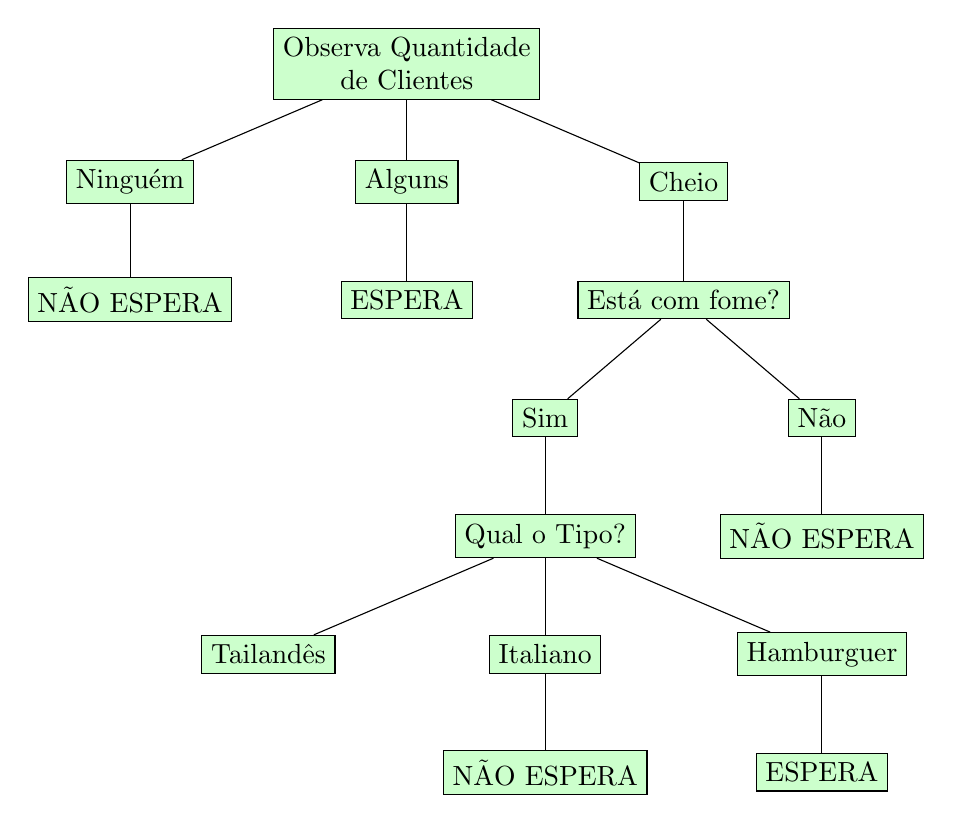
\begin{tikzpicture}[sibling distance=10em,
    every node/.style = {shape=rectangle, 
      draw, align=center,
      top color=green!20, bottom color=green!20}]]
    \node {Observa Quantidade \\ de Clientes}
        child { node {Ninguém} child { node {NÃO ESPERA}  } }
        child { node {Alguns} child { node {ESPERA}  } }
        child { node {Cheio} child { 
            node {Está com fome?} 
            child { node {Sim} child { node {Qual o Tipo?} 
                 child { node {Tailandês} }   
                 child { node {Italiano}  child { node {NÃO ESPERA}  }  } 
                 child { node {Hamburguer} child { node {ESPERA}  } } 
            }   }
            child { node {Não} child { node {NÃO ESPERA}  }  }
            }
        };
  \end{tikzpicture}